%!TEX TS-program = pdflatex

\documentclass[12pt,a4paper,italian]{article} %classe book, A4 con pt 12

\usepackage[utf8]{inputenc} %codifica il documento con UTF8
\usepackage[italian]{babel}
\usepackage{amsmath} %Arricchisce la scelta nel comporre le formule.
\usepackage{amssymb} %idem
\usepackage{graphicx} %facilita la gestione delle figure
\usepackage{amsfonts}
\usepackage{float} %metto le immagini dove voglio
\usepackage{pdfpages} %per il frontespizio
\usepackage[bottom]{footmisc} %note correttamente a pie di pagina
\usepackage[binary-units=true]{siunitx} %unità di misura
\usepackage{textcomp} %marchio registrato, riservato
\usepackage{minted} %comandi bash
\usepackage{eurosym} %simbolo dell'euro

\graphicspath{ {images/} } %le immagini sono nella cartella images
\pagestyle{plain} %lascia vuota la testata e mette il numero di pagina centrato nel piede

\author{Stefano Orioli}
\title{Sistemi flessibili per la cattura di traffico bluetooth}
\date{14/02/2018}




\begin{document}

%\maketitle %stampo il titolo

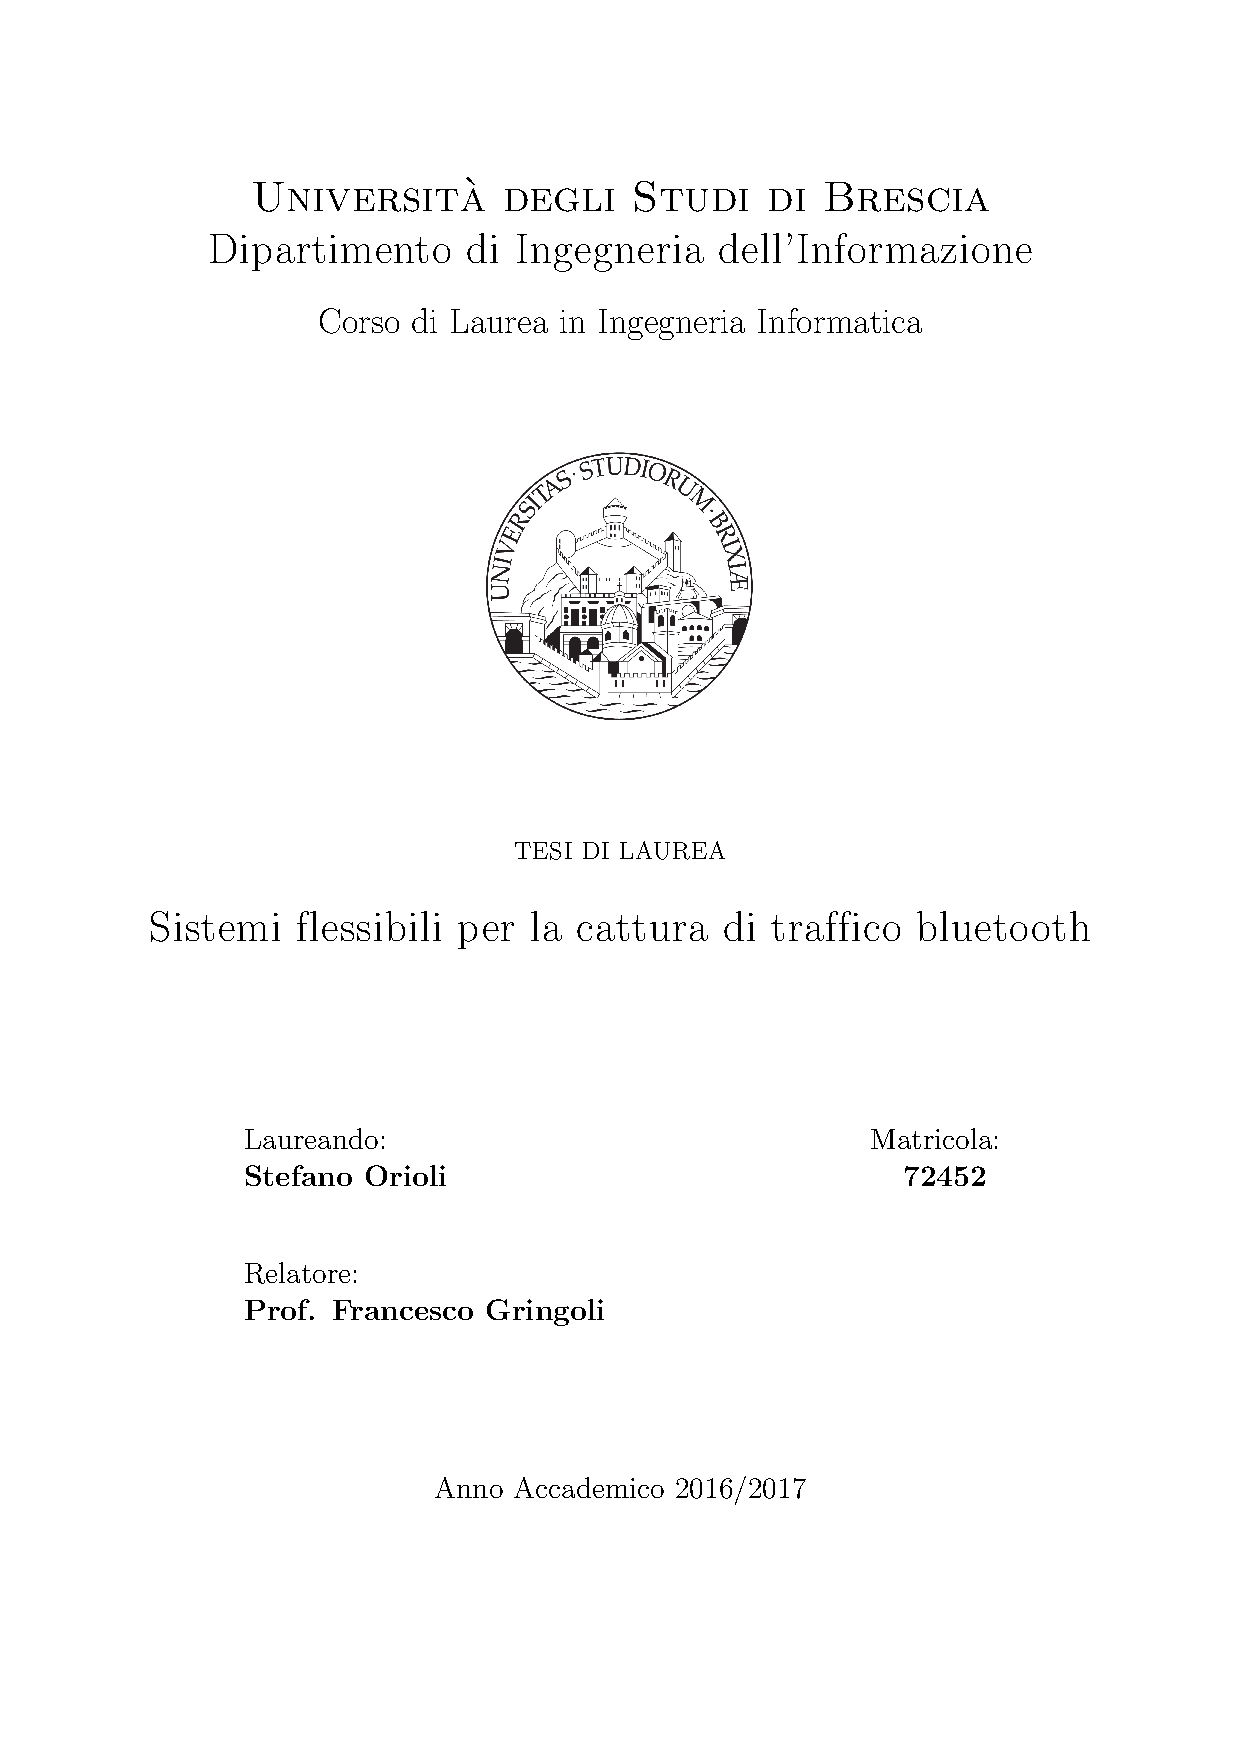
\includepdf{frontespizio}

\newpage 

\tableofcontents %stampo l'indice

%!TEX root = Tesi.tex

\section{Introduzione}
Il Bluetooth è una tecnologia di comunicazione a corto raggio che esiste ormai da parecchi anni sul mercato, ma con l'avvento della specifica Low Energy, introdotta nel 2010 nella versione 4.0 e caratterizzata da un notevole risparmio in termini energetici, è stata adottata da una gran quantità di dispositivi, anche destinati a usi differenti. Basti pensare a tutti quei dispositivi che si definiscono \lq Smart\rq, dalle Televisioni agli Smartphone, dai PC agli orologi, la tecnologia ha un grande impatto sulla nostra vita di tutti i giorni.
Questa rivoluzione comunicativa prende il nome di IoT\footnote{Internet of Things, ovvero l'internet delle cose.}, il mondo dei dispositivi fisici, dove anche il più piccolo di essi, con capacità di calcolo limitate, è in grado di comunicare la propria presenza ed ottenere informazioni sulla rete proprio grazie a queste nuove tecnologie.

\'E quindi corretto chiedersi: queste tecnologie sono sicure? I danni che un malintenzionato sarebbe capace di provocare se riuscisse a manipolare a piacimento il comportamento di questi dispositivi, sono innumerevoli;
Basti pensare ad una serratura intelligente che sblocca la porta di casa quando il proprietario si trova di fronte ad essa, e se non fosse il proprietario quello davanti alla porta, ma tramite un dispositivo di ritrasmissione si spacciasse per esso? Lo stesso discorso si può applicare alle serrature ed al sistema di avvio delle recenti automobili dotate di sistema Keyless\footnote{Senza chiavi, permette l'apertura e l'avvio dell'automobile semplicemente tenendo in tasca le chiavi.}.
Restando in campo informatico, sempre più aziende stanno adottando soluzioni Smart per accedere ai PC, senza dover inserire manualmente la classica password; Apple da la possibilità ai propri utenti di sbloccare il  MacBook tramite il loro Apple Watch, semplicemente avvicinandolo allo schermo; un malintenzionato riuscirebbe con facilità a rubare i dati personali di un utente se riuscisse a sfruttare una falla di questo meccanismo di sblocco.

\'E proprio su questi presupposti che si basa questo progetto di tesi, testare la sicurezza del protocollo Bluetooth tramite la creazione di uno Sniffer a basso costo che permetta di visualizzare ed analizzare i pacchetti scambiati da due dispositivi durante tutta la durata di una connessione. L'implementazione di uno Sniffer è utile anche per un'attività di Debug nello sviluppo delle applicazioni; permette di vedere realmente la composizione del pacchetto inviato e quindi di trovare facilmente errori nell'applicativo.
Uno degli sviluppi futuri è quello riuscire a creare un ripetitore di segnale tra due punti, basandosi sul lavoro svolto in questa tesi, che faccia credere ai dispositivi di essere a stretto contatto quando in realtà li separa una distanza maggiore; questo dimostrerebbe che un dispositivo Bluetooth Low Energy è vulnerabile ad attacchi di tipo Relay, e forzerebbe i costruttori a risolvere queste vulnerabilità e quindi a migliorare la sicurezza del protocollo.

\newpage 

\section{Sistemi esistenti}
Sul mercato esistono già prodotti di sniffing completi, funzionanti e pronti per essere usati; il problema di questi dispositivi è che sono costosi e per la maggior parte non Open Source. La principale limitazione di ciò è che il codice su cui si basano non può essere manipolato a piacimento secondo le proprie esigenze e quindi questi programmi possono essere unicamente usati per lo scopo per cui sono stati creati. Se uno sviluppatore in possesso di uno di questi dispositivi a Closed Source volesse cambiare un leggero aspetto di un programma di Sniffing preconfezionato dovrebbe riscriversi completamente il codice da zero, con un enorme dispendio di tempo e risorse per simulare il comportamento di un applicativo già esistente.

\subsection{Ubertooth One}
Ubertooth One è un progetto Open Source di sviluppo su reti Wireless, capace di comunicare utilizzando il protocollo trasmissivo BLE. Sulla loro pagina GitHub \cite{ubertooth_github_web} è possibile reperire, oltre ai vari progetti sviluppati appositamente, anche il disegno delle componentistiche Hardware, per poter assemblarlo e costruirlo privatamente o addirittura modificarlo secondo le proprie necessità.

\begin{figure}[H]
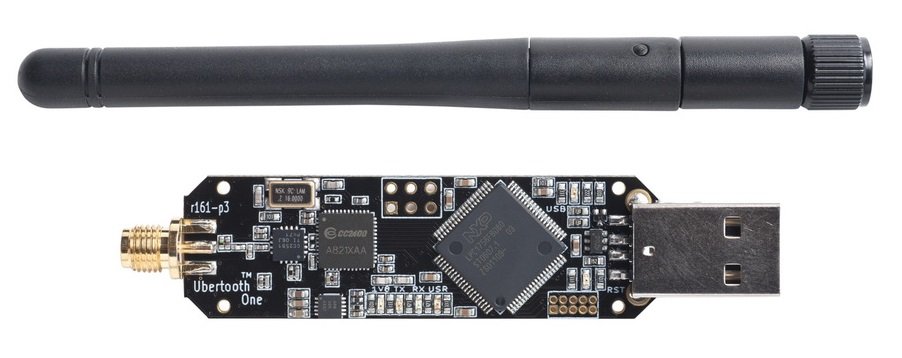
\includegraphics[width=340pt]{ubertooth_one}
\centering
\caption{UberTooth One}
\end{figure}

Si hanno ha disposizione vari progetti creati per questo dispositivo, tra i tanti va citato \lq Bluetooth Captures in PCAP\rq  \cite{ubertooth_pcap_web} che permette di ascoltate, in una sorta di modalità promiscua, tutte le comunicazioni bluetooth su un certo canale, oppure tramite l'ascolto di una CONNECT\_ REQ. seguire una connessione. Permette ulteriormente di interfacciarsi con l'applicazione \emph{WIRESHARK}\footnote{\'E un software per analisi di protocolli o pacchetti utilizzato per la soluzione di problemi di rete, per l'analisi e lo sviluppo di protocolli o di software di comunicazione.} per visualizzare in tempo reale il traffico BLE, applicare filtri su indirizzi o potenza del segnale ed inviare pacchetti personalizzati.

L'aspetto negativo di questa soluzione sta nel costo, difatti ad oggi si trova in commercio ad un prezzo che si aggira attorno ai 150\euro\  + spese di consegna \cite{ubertooth_reseller_web}.

\subsection{Bluefruit LE sniffer}
Il Bluefruit LE monta al suo interno il chip della Nordic nRF51822 che viene venduto già programmato con un software che trasforma il dispositivo in uno sniffer di traffico Bluetooth Low Energy. I pacchetti raccolti vengono mandati in automatico a Wireshark  dove possono essere visualizzati con un'opportuna struttura che facilita la comprensione delle varie parti del pacchetto, senza far riferimento al manuale Bluetooth Core.

\begin{figure}[H]
\includegraphics[width=320pt]{bluefruit_sniffer}
\centering
\caption{Bluefruit LE Sniffer - Bluetooth Low Energy (BLE 4.0) - nRF51822}
\end{figure}

Le limitazioni di questa soluzione sono molteplici; il software che viene installato per gestire il dispositivo come sniffer non è open source; il tool che permette l'interfacciamento tra il dispositivo e wireshark esiste solo per l'ambiente windows. Il dispositivo così come è venduto non può essere programmato, necessita infatti di un programmatore esterno, come il J-Link venduto ad un costo che si aggira sui 15\euro .
Il costo del dispositivo è di circa 25\euro\ paragonabile al prezzo di acquisto di un RedBear Nano2.

\newpage 

\subsection{nRF52 DK}\label{nordic_board}
La board di sviluppo nRF52 DK della Nordic Semiconductor è una periferica di sviluppo versatile e completa per testare applicazioni BLE, ANT e protocolli proprietari che usano le frequenze 2.4GHz. Integra 4 led e 4 bottoni che possono essere usati rispettivamente per ricevere informazioni sullo stato di funzionamento del dispositivo e per impartire comandi a quest'ultimo.

\begin{figure}[H]
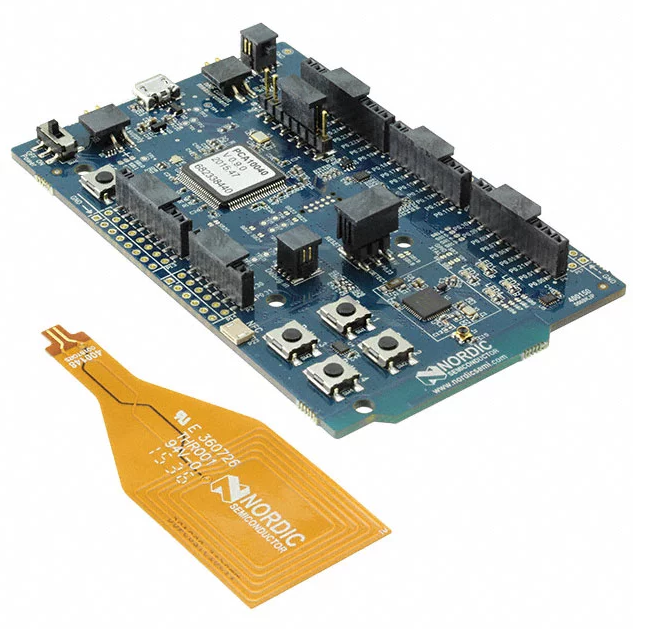
\includegraphics[width=320pt]{nrf52_dk}
\centering
\caption{Board di sviluppo NRF52\_DK creata dalla società Nordic Semiconductor.}
\end{figure}

Essendo ufficialmente supportata dalla stessa Nordic, lo sviluppatore ha a disposizione molti tool per lo sviluppo e il testing di applicazioni. Esiste anche un software di sniffing preconfezionato che permette di svolgere tutte le operazioni di sniffing direttamente da wireshark, tra cui la possibilità di seguire in maniera del tutto automatizzata una connessione e vedere in tempo reale la composizione e il significato di tutti i pacchetti scambiati. 
Sfortunatamente questo software esiste solo per windows e non è open source, quindi non è utilizzabile per lo scopo di questa tesi.
Oltretutto il costo di questa board di sviluppo è di circa 40\euro\ più spese di consegna, più alto di quello di un Nano2.

\subsection{USRP EttusB210}
Il B210 fornisce una singola scheda integrata su una piattaforma USRP\footnote{Universal Software Radio Peripheral, componente della Ettus Research di tipo Software-defined radio (SDR)} con una copertura continua di frequenza da 70 Mhz a 6 GHz. Progettato per la sperimentazione a basso costo, combina il ricetrasmettitore di conversione diretta RFC AD9361 che fornisce fino a 56 MHz di larghezza di banda in tempo reale, un FPGA\footnote{Field Programmable Gate Array, circuito integrato le cui funzionalità sono programmabili via software}, Spartan6 XC6SLX150 open-source e riprogrammabile, ed una connettività ad alta velocità utilizzando USB 3.0 con canale di alimentazione dedicato. Il B210 consente un facile e veloce sviluppo con il toolkit di sviluppo software GNURadio, consentendo così di sperimentare con un'ampia gamma di segnali e bande di frequenza, inclusi trasmissioni FM, TV, cellulari, Wi-fi e Bluetooth.

\begin{figure}[H]
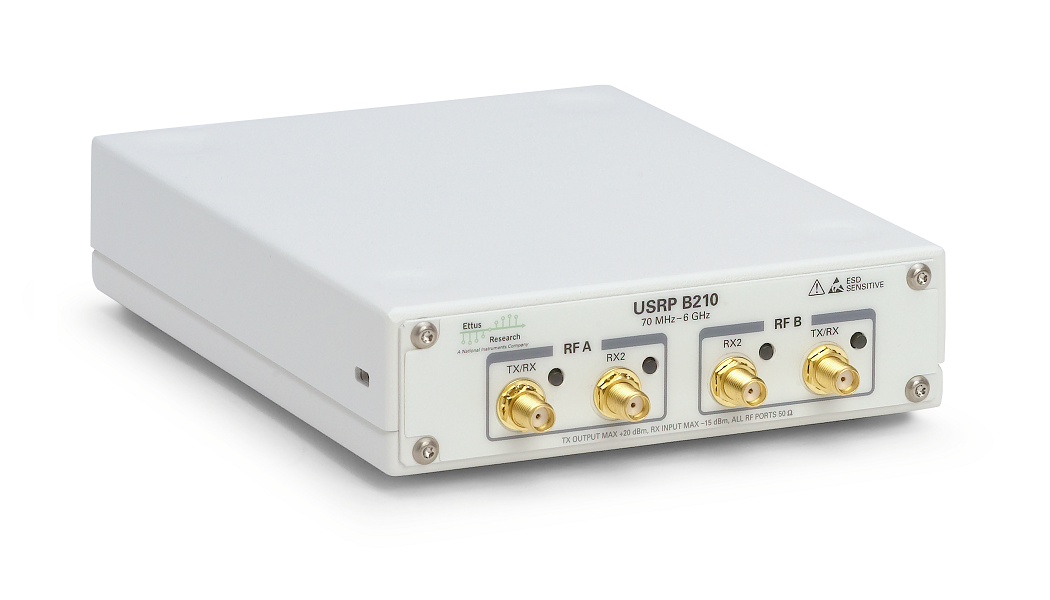
\includegraphics[width=340pt]{usrp_b210}
\centering
\caption{USRP Ettus B210, Ettus Research una società della compagnia National Instrument. }
\end{figure}

La massima banda trasmissiva campionabile in tempo reale con questo dispositivo è di 56 MHz a 61,44 MS/s\footnote{Mega Sample al secondo, unità di misura della frequenza di campionamento.} inferiore alla banda trasmissiva del Bluetooth Low Energy. Il costo di questa board è molto elevato rispetto alle precedenti soluzioni, essendo di circa 1.250\euro\ .
Per questo progetto disponiamo comunque di due di questi dispositivi, essendo stati acquistati dall'università in precedenza, che riescono a coprire gli 80 MHz di banda trasmissiva BLE. Si sono rilevati molto utili per capire ciò che realmente passa nell'etere a quelle frequenze. Il dispositivo campiona qualsiasi segnale nella banda trasmissiva, creando una gran quantità di dati che devono essere poi analizzati e filtrati con un software creato appositamente per estrarne i pacchetti BLE di nostro interesse.

\subsection{Frontline BPA Low Energy}
Progettato e commercializzato dalla società TELEDYNE LECROY, il Frontline BPA Low Energy Bluetooth protocol analyzer è un dispositivo creato appositamente per la funzione di sniffing di pacchetti BLE. Utilizzabile unicamente su sistemi Windows, viene venduto con un applicativo, non open source, da installare che permette di visualizzare tutto il traffico Bluetooth LE in tempo reale, salvare tutto ciò che è stato catturato ed analizzarlo nel dettaglio; con opportuni filtri risulta molto facile trovare il pacchetto di interesse tra gli svariati catturati e vederne nel dettaglio tutte le componenti con i loro valori. \'E interfacciabile anche con WireShark, permettendo quindi all'utente di usufruire delle potenzialità della piattaforma ed integrarlo in progetti già esistenti.

\begin{figure}[H]
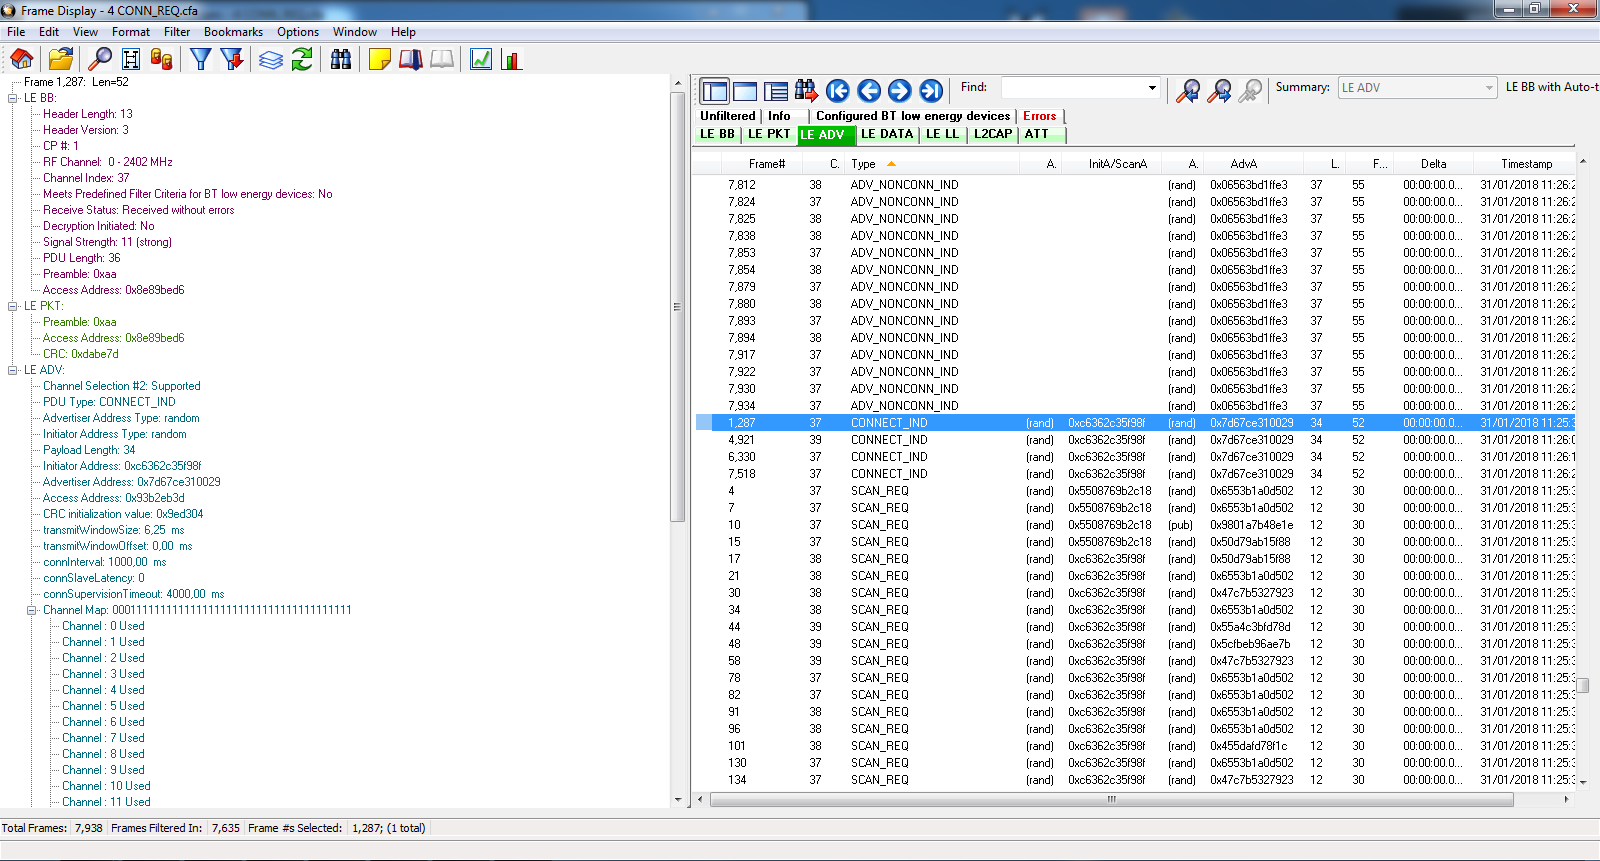
\includegraphics[width=340pt]{frontline_sw}
\centering
\caption{Schermata del software di analisi del traffico ble, distribuito con il dispositivo BPA di sniffing. }
\end{figure}

\'E stato utilizzato come supporto per lo sviluppo del progetto di tesi, in quanto è stato possibile averne uno a disposizione; si è rivelato utile per conoscere esattamente il valore dei vari campi, sopratutto di quelli composti da pochi bit, che il dispositivo nano2 tendeva ad inviare secondo un ordine che non era quello delle specifiche BLE. Conoscendo esattamente il nome del campo ed il relativo valore, fornito dal software di analisi utilizzato con lo sniffer BPA, è stato quindi possibile risalire all'esatta posizione dello stesso all'interno di ciò che veniva catturato dal dispositivo della RedBear, riuscendo a mappare l'esatta disposizione di tutti i campi del pacchetto. Sfortunatamente i documenti che mette a disposizione la società che ha creato il Nano2 sono scarsamente dettagliati e privi di molte informazioni essenziali, si è perciò reso necessario appoggiarsi su strumenti più professionali per capire come funzionasse esattamente e quindi per poter procedere con lo sviluppo di uno Sniffer a basso costo.
Il dispositivo è disponibile sul mercato ad un costo decisamente elevato, che si aggira attorno ai 900\euro\ .

%!TEX root = Tesi.tex

\section{Bluetooth Low Energy}
\subsection{Introduzione}
Il Bluetooth Low Energy (BLE) è una tecnologia wireless introdotta nello standard 4.0, disegnata e commercializzata dal SIG\footnote{Bluetooth Special Interest Group: organizzazione che regolamenta e definisce gli standard  per la trasmissione dati tramite la tecnologia Bluetooth.}; ideata per trasmissioni di dati di breve dimensione, essa si differenzia dal Bluetooth classico per un inferiore consumo di energia, mantenendo la stessa portata trasmissiva.

\subsection{Banda Trasmissiva}
BLE opera alla stessa banda di frequenza del bluetooth classico, 2,400 - 2,4835 GHz, ma utilizza un numero inferiore di canali, 40 canali da 2 MHz l'uno.
Nel canale trasmissivo i dati sono trasmessi con una modulazione GFSK.\footnote{Gaussin Frequency Shift Keying, limita la larghezza dello spettro trasmissivo tramite un filtro di tipo Gaussiano.}
I bitrate trasmissivi sono limitati ai valori 125 kbit/s, 1 Mbit/s o 2 Mbit/s.

Bluetooth Low Energy utilizza il \emph{Frequency Hopping}, una tecnica trasmissiva che consiste nel cambiare canale trasmissivo per ogni pacchetto inviato durante una trasmissione; l'utilizzo di questa tecnica permette di ridurre i problemi di interferenza con gli altri canali ed allo stesso tempo di aumentare la sicurezza delle trasmissioni.

\subsection{Stack protocollare}
Storicamente lo stack Bluetooth è diviso in 2 componenti fondamentali: il \emph{Controller} e l'\emph{Host}.
La parte di Controller è quella che si occupa di eseguire le componenti di basso livello dello stack necessarie per gestire i pacchetti scambiati a livello fisico e le loro temporizzazioni; la parte di Host comprende le componenti di alto livello tra cui profili e API\footnote{Application Program Interface: insieme di procedure utili a svolgere uno specifico compito}. La parte di Host, diversamente da quella di controllo, astrae dall'hardware ed è caratterizzata da una gestione meno rigida delle temporizzazioni.

L'\emph{HCI}\footnote{Host Controller Interface}, l'interfaccia tra Host e Controller si occupa di mettere in comunicazione queste due componenti fondamentali, utilizzando canali comunicativi quali UART o USB.
Se i due componenti sono montati su uno stesso chip, come nel caso dei SoC\footnote{System on a Chip: sistema completamente contenuto su un solo Chip}, allora l'interfaccia HCI è opzionale e può essere omessa.

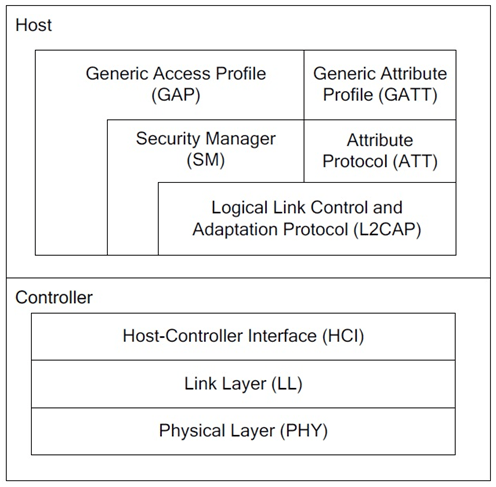
\includegraphics[scale=0.5]{stack_ble.png}

\begin{itemize}
\item Physical Layer (PHY): è il livello fisico, ovvero l'etere; lavora nella banda di frequenza 2,4 GHz ISM\footnote{Industrial, Scientific and Medical: frequenze riservate alle applicazioni di radiocomunicazioni non commerciali, ovvero per uso industriale, scientifico e medico.} Si compone di 40 canali da 2 MHz ognuno suddivisi in 3 per advertising e 37 per lo scambio dati.

\item Link Layer (LL): si occupa della gestione della sequenza e della temporizzazione dei pacchetti scambiati. Dialoga con i nodi vicini e scambia informazioni quali i parametri di connessione e controllo di flusso.\linebreak 
\'E una macchina a stati che si compone di 5 stati: Standby, Advertising, Scanning, Initiating, Connection. 

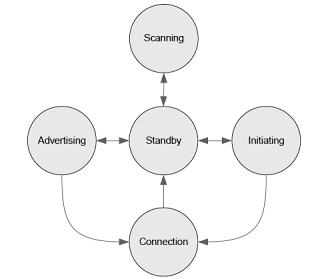
\includegraphics[scale=0.5]{LL_states}

\begin{itemize}

\item Advertising: il dispositivo rende noto agli ascoltatori della propria presenza, indicando la disponibilità ad una connessione ed inviando alcune informazioni utili.

\item Scanning: il dispositivo è in ascolto di tutte le informazioni trasmesse sui canali di advertise.

\item Initiating: un dispositivo in ascolto individua un Advertise di suo interesse ed indica la sua volontà di connettersi.

\item Connection: due o più dispositivi sono connessi.

\item Standby: il dispositivo è in uno stato di attesa caratterizzato da un basso consumo energetico.

\end{itemize}

Lo stato di Scanning può essere attivo (richiede informazioni aggiuntive) o passivo; Lo stato Connection anch'esso si divide in 2 sottostati: Central e Peripheral.

\item Logical Link Control and Adaptation Protocol (L2CAP): fornisce servizi sui dati ai livelli superiori, come ad esempio il Security Manager Protocol o l'Attribute Protocol. \'E responsabile inoltre della segmentazione e ricostruzione dei pacchetti da e verso i livelli inferiori.

\item Security Manager (SM): è responsabile del pairing dei dispositivi e della distribuzione delle chiavi crittografiche; BLE utilizza lo standard AES-128 bit per la cifratura dei dati ed il sistema di pairing per la distribuzione delle chiavi.

\item Attribute Protocol (ATT): gestisce la distribuzione delle informazioni riguardanti le coppie attributo-valore presenti in un device peripheral (Server)

\item Generic Access Profile (GAP): controlla \emph{advertising} e \emph{connection} . Divide i dispositivi bluetooth low energy in:
\begin{itemize}
\item Peripheral: normalmente dispositivi dotati di una limitata capacità di calcolo, come ad esempio un sensore di temperatura.
\item Central: dispositivo che gestisce la rete bluetooth e che richiede una maggiore capacità di calcolo; mentre un dispositivo periferico può avere una connessione con un solo dispositivo centrale, un centrale può gestire più dispositivi periferici andando a creare una Piconet\footnote{Rete Bluetooth composta da massimo otto dispositivi in relazione master-slave e fino a 255 dispositivi in modalità inattiva o parcheggio.}
\end{itemize} 

\item Generic Attribute Profile (GATT): entra in gioco a connessione avvenuta, definisce il modo in cui 2 dispositivi BLE scambiano dati utilizzando i concetti di \emph{Services} e \emph{Characteristics}.

\begin{itemize}
\item GATT server: è un peripheral device, che tramite il protocollo ATT permette al central di conoscere i dati che ha memorizzato in strutture di tipo service-characteristic.
\item GATT client: è il central device, che gestisce le comunicazioni e che richiede ai server periferici i dati raccolti.
\end{itemize}



\end{itemize}



 

%!TEX root = Tesi.tex

\section{RedBear Nano2}
Il dispositivo usato per implementare la funzione di sniffer è il Nano2 della società RedBear. Non più grande di una moneta (10mm x 18mm), ha un costo che si aggira attorno ai 30\$ .

\begin{figure}[H]
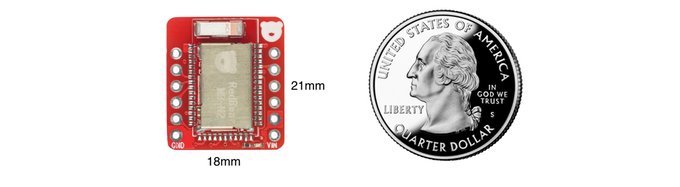
\includegraphics[width=300pt]{nano2_money}
\centering
\caption{RedBear Nano2, comparato con una moneta da 1/4 di dollaro.}
\end{figure}

Il nome in codice del modello è \lq MB-N2\rq ed integra al suo interno il chip della Nordic nRF52832, un'antenna integrata ed un totale di 32 pin di I/O\footnote{Input, Output: utilizzabili a piacimento come periferiche di ingresso o uscita} che offrono i servizi di UART, SPI, ADC e PWM.

\begin{figure}[H]
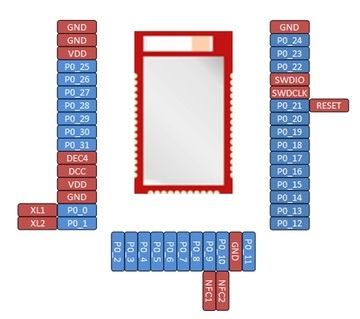
\includegraphics[width=250pt]{nano2_io}
\centering
\caption{Modulo SoC Nordic nRF52832 integrato nel RedBear Nano2.}
\end{figure}

\begin{samepage}
Il chip della Nordic Semiconductor nRF52832 Soc ha le seguenti caratteristiche
\begin{itemize}
\item[-] Processore ARM Cortex-M4F a 32 bit e 64 MHz.
\item[-] Bluetooth 4.2 certificato e compatibile con le specifiche 5.0 .
\item[-] NFC.
\item[-] 64 KB di ram.
\item[-] 512 KB di memoria Flash.
\item[-] FPU, unità di calcolo in virgola mobile.
\item[-] DSP, processore di segnale digitale.
\end{itemize}
\end{samepage}

Non disponendo di un'interfaccia standard per la comunicazione con un PC, il Nano2 necessita di una board di supporto sia per essere programmato, sia per comunicare informazioni a quest'ultimo.
La board che viene fornita assieme al Nano2 è chiamata DAPLink e disponibile nella versione 1.5 . Essa monta un processore ARM Cortex-M3 MCU ed è utilizzata oltre che per la programmazione, anche per il debug dei progetti su Nano2

\begin{figure}[H]
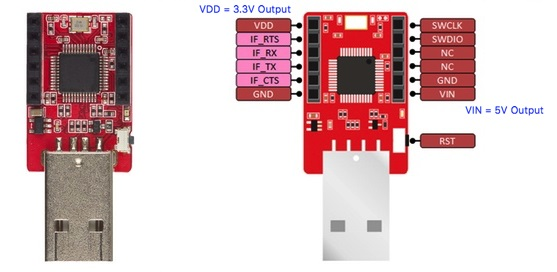
\includegraphics[width=330pt]{daplink}
\centering
\caption{Board DAPLink, un progetto open source del team ARM mbed.}
\end{figure}




%!TEX root = Tesi.tex

\section{Ambiente di sviluppo}
\subsection{Introduzione}
\'E stato scelto di sviluppare l'intero progetto di tesi in ambiente UNIX, usando come sistema operativo Linux, nello specifico la distribuzione di Ubuntu 17.04 a 64 bit denominata Zesty Zapus. Questa decisione è stata presa per integrare al meglio i progetti ed il codice già esistente e per creare una base di sviluppo futura che sia Open Source\footnote{Qualità di un sistema che consiste nell'essere di libero uso e riutilizzabile senza alcun costo, per ampliarne funzionalità e caratteristiche} e liberamente utilizzabile senza alcun vincolo di licenza. Non è stata comunque una decisione immediata perché il RedBear Nano2 integra un Soc\footnote{Sistem on a Chip, è un particolare circuito integrato che in un solo chip contiene un sistema completo} progettato dalla società Nordic Semiconductor, chiamato \lq\lq nRF52832\rq\rq, la quale mette a disposizione vari Tool, funzionalità e IDE di sviluppo per questo chip ideati e creati  per funzionare unicamente in ambiente Windows; fortunatamente esistono vari progetti e guide abbastanza dettagliate reperibili online, alcune delle quali supportate direttamente dalla Nordic stessa, che aiutano a settare ed integrare il materiale già esistente anche in ambiente UNIX.
Rimangono comunque delle forti limitazioni nello sviluppo degli applicativi per Nano2 su Linux, primo fra tutti la mancanza della possibilità di un ambiente di Debug che permetta l'analisi istruzione per istruzione del codice in esecuzione sul dispositivo, con la relativa possibilità di visualizzazione dei valori delle varie variabili durante l'esecuzione; questa limitazione è stata in parte sopperita utilizzando l'interfaccia UART, utilizzandola per inviare stringhe contenenti informazioni su quali parti del codice fossero o meno state realmente eseguite ed il valore di alcune variabili di interesse nelle varie fasi dell'esecuzione dell'applicativo sviluppato. 
Questa incompatibilità ha rallentato il processo di sviluppo su Linux ma non lo ha reso impossibile, ne tanto meno ne ha limitato le potenzialità.

\subsection{Installazione GNU toolchain}\label{inst_gnu_toolchain}
Prima di iniziare a scrivere codice, è necessario installare dei componenti software che permettano di compilare in linguaggio macchina ARM il codice da noi prodotto.
Quello che ci serve è un compilatore chiamato \emph{GNU toolchain for ARM Cortex-M} scaricabile gratuitamente dal sito ufficiale di \lq arm.developer\rq. \cite{armweb} Una volta scaricato ed estratto il pacchetto, bisognerà aggiungere al PATH di sistema la seguente directory:

\begin{minted}{bash}
<directory estratta>/gcc-arm-none-eabi-6-2017-q2-update/bin
\end{minted}

Per compiere questa operazione in Ubuntu, basterà aprire una finestra del terminare BASH ed eseguire il comando:

\begin{minted}[breaklines]{text}
echo 'export PATH=\$PATH:<directory estratta>/gcc-arm-none-eabi-6-2017-q2-update/bin' >> ~/.profile 
\end{minted}

ovvero aggiungere al file .profile il percorso al compilatore, il quale sarà aggiunto poi in automatico alla variabile di sistema PATH; questo permetterà di invocare i comandi di compilazione da qualunque punto del sistema, senza dover richiamare il percorso al compilatore.
\'E possibile verificare se il procedimento è stato eseguito con successo eseguendo il seguente comando al terminale:

\begin{minted}{bash}
arm-none-eabi-gcc --version
\end{minted}
che deve restituire la versione del compilatore installata.

Un altro componente essenziale da aver installato è il compilatore \emph{GNU make}, che normalmente è già presente sulla maggior parte delle distribuzioni UNIX. Se così non fosse, per quanto riguarda Ubuntu, si installa semplicemente eseguendo il comando:

\begin{minted}{bash}
sudo apt-get install build-essential checkinstall
\end{minted}

\subsection{Configurazione SDK}
L'SDK\footnote{Software Development Kit}, ovvero l'insieme di tutte le funzioni di libreria necessarie per creare applicazioni da eseguire sul Nano2, è liberamente scaricabile dal sito della Nordic Semiconductor \cite{sdkweb} ; La versione utilizzata per questo progetto è la 14.1.0 che è creata per essere utilizzata sul Chip nRF52832.
La struttura di questa SDK è molto rigida, tutti i progetti contenuti al suo interno fanno riferimento ai vari file contenuti nell'SDK con un percorso assoluto; è meglio quindi non modificarne la struttura per non avere problemi di compilazione in futuro.
Scaricata ed estratta in una directory a piacimento, va impostato il percorso alla toolchain ARM, installata nel capitolo \ref{inst_gnu_toolchain}, andandolo a impostare nel file makefile.posix che si trova nella cartella: 

\begin{minted}{text}
<SDK>/components/toolchain/gcc
\end{minted}
dove \textless SDK\textgreater  è la root dell'SDK estratto.

Aprendo il file con un semplice editor di testo, cambiare i 3 campi riportati come segue:

\begin{minted}{text}
GNU_INSTALL_ROOT := .../gcc-arm-none-eabi-6-2017-q2-update/bin/
GNU_VERSION := 6.3.1
GNU_PREFIX := arm-none-eabi
\end{minted}

Nella SDK si trovano anche molti progetti di esempio, da cui è essenziale partire per sviluppare un nuovo programma; ogni progetto di esempio contiene svariati file sorgente da compilare e linkare. Per rendere semplice la compilazione è fornito un Makefile, ovvero un file che contiene tutte le istruzioni per la compilazione del progetto e che integra regole di dipendenza e regole di interpretazione, utilizzate per conoscere quali sono i file utilizzati nel progetto, con il relativo percorso, garantendo una compilazione esente da errori e solo di quei file sorgente che sono stati modificati dall'ultima compilazione.

Da questo punto è possibile compilare un progetto di esempio direttamente da terminale, per verificare che i passi compiuti fin'ora siano stati eseguiti correttamente; portandosi nella cartella del progetto \lq blinky\rq e successivamente nella sotto cartella \emph{armgcc}; qui invocando il comando \emph{make} si avvierà la compilazione che se avrà successo creerà una sotto cartella chiamata \_build contenete il file nrf52832\_xxaa.hex, che è il nostro programma compilato in linguaggio macchina ARM che dovrà essere poi scritto sulla memoria del Nano2 per essere eseguito.
Per scrivere il file sulla memoria del Nano2 basterà copiarlo all'interno della periferica usb che viene rilevata dal pc quando lo si connette tramite la board DAPLink v1.5 .
\subsubsection{Configurazione piedinatura Nano2}
Il dispositivo della società RedBear chiamato Nano2 che viene utilizzato in questa tesi, non è uno dei dispositivi ufficialmente supportati dalla SDK; Bisogna quindi prendere una delle varie board che vengono ufficialmente supportate e cambiarne la piedinatura, ovvero l'associazione tra una specifica periferica, come il led, o una specifica funzionalità, ad esempio UART, e il relativo pin sul chip. 
\'E stato scelto di prendere la board di sviluppo PCA10040 ed il relativo file di configurazione pca10040 e adattarne la piedinatura con quella dichiarata dalla Redbear, mostrata in figura \ref{nano2_pins}

\begin{figure}[H]
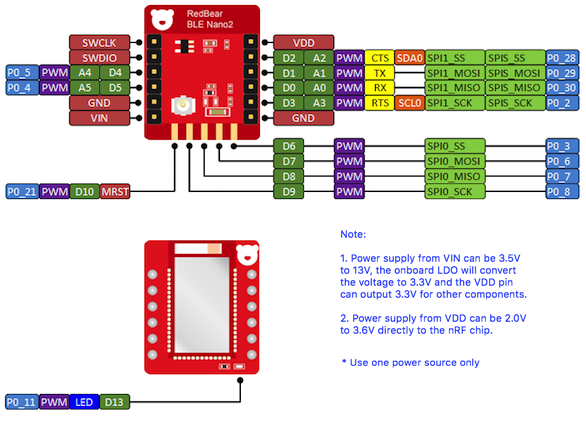
\includegraphics[width=400pt]{nano2_pins}
\centering
\caption{Piedinatura del modulo Nano2}
\label{nano2_pins}
\end{figure}
ad esempio, qui si ha a disposizione solo 1 led, connesso al pin 11, mentre sulla board PCA10040 se ne avevano 4. Bisognerà cambiare quindi il numero totale di led da 4 a 1 ed il pin dell'unico led con il valore 11.
Dopo aver modificato correttamente questo file, tutte le modifiche saranno automaticamente aggiornate per tutti gli esempi contenuti nell'SDK, andando a selezionare per ogni progetto il makefile contenuto nella cartella che riporta il nome della board PCA10040.
Per l'esempio del lampeggio del led, il percorso per raggiungere il makefile corretto sarà quindi:

\begin{minted}{text}
<SDK>/examples/peripheral/PCA10040/blank/armgcc/
\end{minted}

\subsubsection{Softdevice}
Progetti più complessi di un semplice lampeggio di un led, come tutti i progetti che permettono lavorare con il BLE, necessitano che assieme al codice del programma venga scritto sul dispositivo dell'altro codice preconfezionato; questo ulteriore codice, chiamato \emph{Softdevice} non è altro che un insieme di funzioni di libreria che vengono fornite già compilate e che sono utilizzabili dal nostro codice per svolgere le operazioni più complesse utilizzando poche righe di codice. Esistono varie versioni del softdevice, diverse per funzionalità e compatibilità con i chip; per tutti le applicazioni sviluppate è stata usata la versione S132.
Se si sta sviluppando un progetto che utilizza tali funzioni, prima di andare a scrivere il file .hex sul Nano2 bisognerà unirlo con il softdevice, che viene fornito nella SDK (<SDK>/components/softdevice/s132/hex), utilizzando una utility scaricabile dal sito della Nordic, chiamata \lq mergehex\rq, e disponibile per tutti i Sistemi Operativi.
Per velocizzare il processo di unione dei due file .hex e successiva scrittura sul Nano2 è stato creato uno script di bash che automatizza tutto il processo:

\begin{minted}{text}
#!/bin/bash

SOFTDEVICE=/home/utente/SoftDevices/s132_nrf52_5.0.0/s132_nrf52_5.0.0.hex
SORGENTE=nrf52832_xxaa.hex 
OUTPUT=toflash.hex
USB_PROG=/media/utente/DAPLINK

mergehex -m ${SORGENTE} ${SOFTDEVICE} -o ${OUTPUT}

echo "Flashing to ${USB_PROG} ..."
cp ./${OUTPUT} ${USB_PROG}/{OUTPUT}
\end{minted}

\subsection{Installazione IDE}
Anche se non strettamente necessario ai fini dello sviluppo, un ambiente grafico per la scrittura del codice (IDE) è consigliato, dato il gran numero di righe di codice che può contenere un applicativo. Eclipse, l'IDE di sviluppo utilizzato in questa tesi, è un ambiente di sviluppo integrato multi-linguaggio e multipiattaforma sviluppato in Java dalla \emph{Eclipse Foundation}, distribuito liberamente e gratuitamente.
Oltre all'ide di base, nella versione per sviluppatori C,C++ vanno aggiunti vari pacchetti per permettere lo sviluppo sui dispositivi integrati con processore ARM; per facilitare le operazioni di aggiunta e settaggio di questi pacchetti esistono delle versioni di Eclipse modificate che integrano tutti questi pacchetti; queste versioni modificate è scaricabile gratuitamente dal repository GitHub \emph{gnu-mcu-eclipse} \cite{gnueclipseweb}. Scaricato ed estratto in una directory a piacimento sarà già pronto per essere utilizzato per sviluppare applicazioni per il Nano2.
\subsubsection{Importare un esempio in Eclipse}
Per inziare a sviluppare o testare uno dei vari esempi presenti nell'SDK utilizzando Eclipse, bisogna prima importarlo nell'ambiente di lavoro. 
Per fare ciò bisogna creare un nuovo progetto in Eclipse che si basi su un Makefile esistente.

\begin{minted}{text}
File -> Makefile Project with Existing Code
\end{minted}
andando poi a impostare come percorso la cartella che contiene il makefile del progetto; come toolchain bisognerà settare \lq ARM Cross GCC\rq .

\begin{figure}[H]
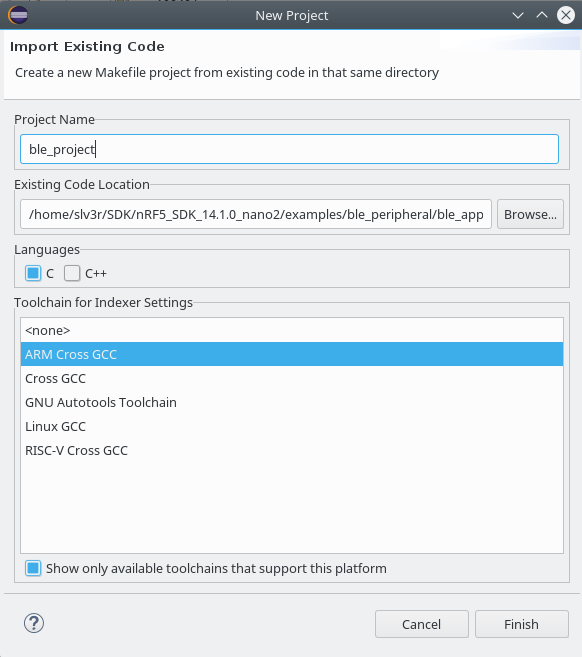
\includegraphics[width=300pt]{new_makefile_project}
\centering
\caption{Creazione di un nuovo progetto da Makefile}
\label{makefile_proj}
\end{figure}

Nella schermata dei progetti di eclipse apparirà il progetto appena creato, vedremo però solo il file Makefile; si deve importare manualmente il file main.c andando prima a creare una nuova cartella virtuale, tramite il percorso \mbox{New-\textgreater  Folder} e nella schermata selezionare Advanced e successivamente Virtual Folder. Poi tramite tasto destro sulla \mbox{cartella-\textgreater  import} andare a selezionare il file main.c che è situato nella cartella principale del progetto.

\begin{figure}[H]
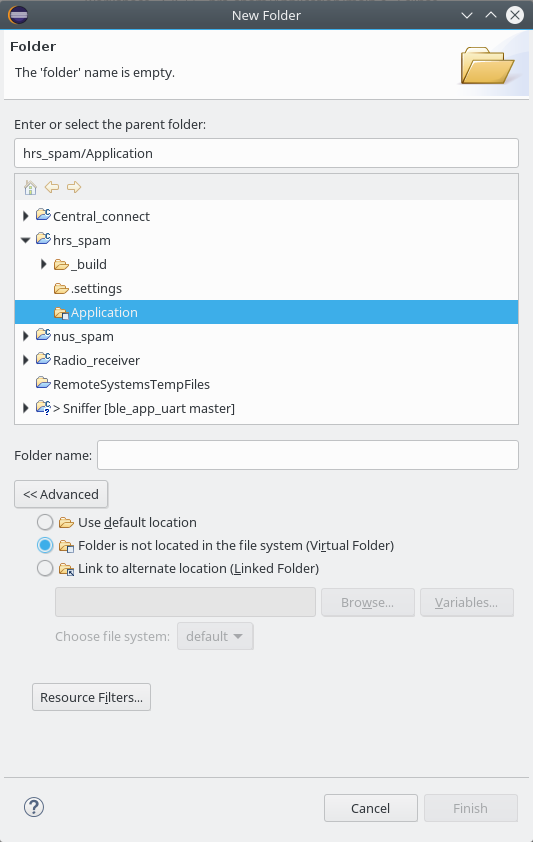
\includegraphics[width=270pt]{new_folder_eclipse}
\centering
\caption{Creazione di una cartella virtuale nel progetto, che conterrà il file main.c}
\label{makefile_proj}
\end{figure}

\begin{samepage}
L'ultima operazione da compiere prima di poter compilare tramite Eclipse è settare il comando di compilazione; tramite tasto destro sulla cartella del progetto, visualizzata a lato sinistro, e selezionando Properties. Si aprirà una nuova schermata in cui si deve selezionare C/C++ Build ed impostare il campo Build Command come segue: 

\begin{minted}{text}
make VERBOSE=1
\end{minted}
\end{samepage}

Questo, oltre ad invocare il comando corretto di compilazione, crea un output di tipo \lq verbose\rq dal quale Eclipse ottiene le informazioni sui percorsi dei vari file da cui dipende il main, andando quindi ad eliminare tutti gli errori sintattici che erroneamente l'IDE evidenzia.

\begin{figure}[H]
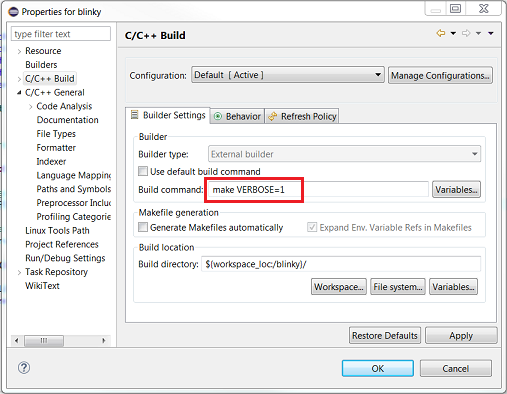
\includegraphics[width=350pt]{verbose_eclipse}
\centering
\caption{Impostazione del comando di compilazione su Eclipse}
\end{figure}



%!TEX root = Tesi.tex

\section{Progettazione sniffer}
Il primo passo per lo sviluppo è stato prendere confidenza sia con l'ambiente di lavoro che con il dispositivo della RedBear. Testare un semplice progetto, come il lampeggio di un led, si è comunque rivelata un'operazione non banale.
L'SDK che la Nordic fornisce contiene esempi modificati appositamente per le sue board di sviluppo, come la PCA10040 o la PCA10056, descritte nel capitolo \ref{nordic_board}, che come già accennato hanno una piedinatura e una dotazione di periferiche differente rispetto al nano2. Il primo passo è stato quindi quello di utilizzare una board supportata e modificarne la piedinatura delle periferiche connesse; il numero di led è stato ridotto a 1 solo connesso al pin 11 e sono stati rimossi i riferimenti a pulsanti connessi, perché non presenti sulla nostra periferica. \'E stato necessario modificare anche i collegamenti dei 4 pin relativi alla comunicazione UART come segue:
\begin{itemize}
\item[-] CTS pin 28
\item[-] RTS pin 2
\item[-] TX pin 29
\item[-] RX pin 30
\end{itemize}
Tutte queste modifiche sono state apportate al file pca10040.h che si trova nell'sdk nella cartella /components/boards .

Eseguendo una nuova compilazione e provando a scrivere il file .hex generato continuava a non funzionare. Dopo varie prove si è capito che mancavano delle librerie da cui il progetto dipendeva; esse sono contenute nel SOFTDEVICE, un file .hex che viene fornito già compilato nell'SDK, nella cartella /components/softdevice/s132/hex. Per tutti i progetti creati si usa la versione s132 del softdevice che è la più completa e contiene tutte le librerie necessarie per far funzionare il nano2 sia come dispositivo di tipo central che peripheral.

\subsection{UART}
Per visualizzare i dati intercettati via etere è necessario poter comunicare informazioni ad un dispositivo dotato di output video; nel nostro caso è stato utilizzato un PC, che avendo una gran capacità di memorizzazione può contenere tutti i dati catturati, per essere visualizzati ed analizzati anche in un secondo momento. Per trasferire questi dati abbiamo utilizzato una funzionalità supportata dal nano2, la trasmissione usando UART. \'E l'acronimo di Universal Asynchronous Receiver Transmitter, ovvero ricevitore trasmettitore asincrono/seriale, è un dispositivo hardware che converte flussi da un formato parallelo, tipicamente quelli usati all'interno di un processore, in formato seriale asincrono.
Inviare dati tramire UART è un'operazione che richiede pochi settaggi e quindi poche righe di codice, utilizzando le apposite funzioni di libreria messe a disposizione nella SDK. 

\begin{samepage}
All'interno di un progetto, va prima inizializzato il modulo fornendo le impostazioni che desideriamo usare:
\begin{itemize}
\item[-] Baudrate: il numero di simboli che vengono trasmessi in un secondo, determina la velocità di trasmissione.
\item[-] Control Flow: indica se utilizzare o meno le due linee aggiuntive destinate alla comunicazione UART ovvero, CTS (Clear To Send) e RTS (Ready To Send) per gestire lo scambio di dati, utile per annullare i conflitti trasmissivi.
\end{itemize}
Normalmente i settaggi sono inseriti nella funzione \emph{uart\_init()} che viene eseguita all'avvio del dispositivo.
\end{samepage}

Vanno inseriti dei caratteri di controllo per differenziare la fine di un pacchetto con l'inizio del successivo, ed eventualmente indicare informazioni aggiuntive al solo pacchetto, come la lunghezza dello stesso. \'E quindi stato inserito il carattere denominato MARKER del valore di 0xE0 all'inizio di ogni dato inserito; i 2 Byte successivi indicano la lunghezza dell'intero pacchetto, quindi comprendono anche i caratteri di controllo. Il quarto Byte viene usato per indicare il canale il cui è stato catturato il pacchetto e dal 5° Byte in poi si avrà ciò che è stato catturato, così come viene rilevato dal Nano2.
\begin{figure}[H]
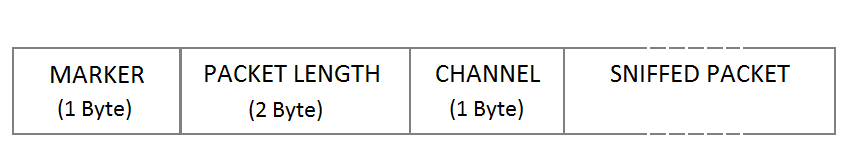
\includegraphics[width=300pt]{uart_packet}
\centering
\caption{Pacchetto inviato tramite UART che contiene il pacchetto sniffato e i campi di controllo.}
\end{figure}
Nel caso in cui all'interno del pacchetto stesso ci siano Byte del valore di 0xE0, che hanno lo stesso valore del Marker, per evitare di confonderli si raddoppia il Byte. In questo modo se nel pacchetto ricevuto si incontrerà un Byte singolo del valore del Marker, allora quello sarà un vero Marker che indica l'inizio di una nuova trasmissione; negli altri casi sarà un Byte del pacchetto, si dovrà quindi scartare il Byte successivo, che non fa parte dei dati catturati dallo Sniffer.

\subsection{NRF RADIO}



%!TEX root = Tesi.tex

\section{Bibliografia}

\begin{thebibliography}{9}

\bibitem{bt_core_v4} 
Bluetooth SIG Working Groups. 
\textit{Bluetooth\textsuperscript{\textregistered} Core Specification v4.0}
\mbox{30 June 2010}.

\bibitem{adafruitweb} 
Introduction to Bluetooth Low Energy, 
\\\texttt{https://learn.adafruit.com/introduction-to-bluetooth-low-energy}
 
\bibitem{dmitryweb} 
CRC and data whitening, 
\\\texttt{http://dmitry.gr/index.php?r=05.Projects\&proj=11.\% 20Bluetooth\%20LE\%20fakery}

\bibitem{eetimesweb} 
Bluetooth LE Stack Partition, 
\\\texttt{https://www.eetimes.com/document.asp?doc\_id=1278966}

\bibitem{armweb} 
Bluetooth LE Stack Partition, 
\\\texttt{https://developer.arm.com/open-source/gnu-toolchain/gnu-rm/downloads}

\bibitem{sdkweb} 
Bluetooth LE Stack Partition, 
\\\texttt{http://developer.nordicsemi.com/nRF5\_SDK/nRF5\_SDK\_v14.x.x}

\bibitem{gnueclipseweb} 
GNU MCU Eclipse IDE for C/C++ Developers Neon, 
\\\texttt{https://github.com/gnu-mcu-eclipse/org.eclipse.epp.packages/releases/}


\end{thebibliography}

\end{document}\grid
\grid
